% =============================================================================
% RESULTS - CITA Paper in ALKALI Format
% =============================================================================





\vspace{-0.5mm}
\section{Experiments \& Results}
\label{sec:results}

\textls[0]{We evaluate whether \textsc{CITA} supports \emph{instruction-conditioned behavioral switching}—a \textbf{policy-level} change under a fixed user prompt—rather than merely inducing \emph{surface-form compliance}. Our study spans \textbf{5 benchmarks} and \textbf{10 model variants}, enabling a controlled comparison of both \emph{base performance} and \emph{instruction sensitivity}. Unless noted otherwise, we report \textbf{deterministic, non-LLM metrics} to reduce evaluator drift and improve reproducibility, consistent with holistic evaluation practice~\cite{liang2023holistic,sun2024trustllm}. Across this suite, \textsc{CITA} attains \textbf{\colorbox{bg-green}{95.6\%}} instruction-alignment efficiency, surpassing \textsc{DPO} (70.5\%) by \textbf{+25.1 pp} and outperforming \textsc{GRPO}/\textsc{PPO}/\textsc{SFT} by wider margins.}


\vspace{-2mm}
\subsection{Training Pipeline}
\label{sec:training_pipeline_exp}

\noindent\textbf{Setup.} Following the staged pipeline from \cref{sec:methodology}, we train on PKU-SafeRLHF~\cite{ji2024pku,bai2022training} using NVIDIA A100 GPUs with LoRA adapters~\cite{hu2022lora} (SFT/DPO/CITA on A100-40GB; PPO/GRPO on A100-80GB due to online generation overhead). Training proceeds through four stages: \vspace{-1mm}
\begin{enumerate}[leftmargin=*,itemsep=0pt]
    \item \textbf{Base:} Llama-3.1-8B pretrained weights~\cite{dubey2024llama}
    \item \textbf{SFT:} fine-tune on PKU \emph{chosen} responses
    \item \textbf{DPO:} \textls[0]{preference optimization on PKU preference pairs}
    \item \textbf{CITA:} instruction-conditioning + \textbf{mandatory} KL anchoring
\end{enumerate}
\vspace{-1em}


\paragraph{Training Dynamics}
\label{sec:training_dynamics}

\noindent We track training curves for preference separation and stability. \Cref{fig:training_margins} reports reward margins, where larger values indicate stronger separation between preferred and dispreferred responses under the learned objective.

\vspace{-0.35em}
\paragraph{Training pipeline (stability-first).}
We separate \textbf{format competence} from \textbf{instruction-conditioned preference geometry}:
\textbf{Base $\rightarrow$ SFT} to stabilize instruction-following priors and response formatting; then \textbf{SFT $\rightarrow$ CITA} to learn the conditional preference field under a KL-shaped trust region (cf. Appendix \ref{sec:training_pipeline_exp}).
%\noindent\textbf{Rationale.} The \textsc{CITA} stage is designed to preserve a stable policy manifold under instruction switches via explicit anchoring, rather than relying on implicit regularization.

\vspace{-2mm}
\subsection{Model Variants $\times$ Alignment Methods}
\label{sec:model_variants}

\textls[0]{\noindent We train \textbf{10 variants} across \textbf{5 methods} (\textsc{SFT}, \textsc{PPO}, \textsc{GRPO}, \textsc{DPO}, \textsc{CITA}) $\times$ \textbf{2 instruction settings}: \textbf{NoInstruct} (standard prompts) vs.\ \textbf{Instruct} (prompts augmented with behavioral instructions). This enables a controlled estimate of each method’s \textbf{instruction sensitivity} (Instruct $-$ NoInstruct) and separates \emph{instruction robustness} from raw base performance.}

% \vspace{-1.5mm}
% \begin{table}[H]
% \centering
% \footnotesize
% \setlength{\tabcolsep}{6pt}
% \begin{tabular}{@{}lll@{}}
% \toprule
% \textbf{Model} & \textbf{Training Path} & \textbf{Instruction} \\
% \midrule
% SFT\_NI & Base$\rightarrow$SFT & No \\
% SFT\_I & Base$\rightarrow$SFT & Yes \\
% \midrule
% PPO\_NI & Base$\rightarrow$SFT$\rightarrow$PPO & No \\
% PPO\_I & Base$\rightarrow$SFT$\rightarrow$PPO & Yes \\
% \midrule
% GRPO\_NI & Base$\rightarrow$SFT$\rightarrow$GRPO & No \\
% GRPO\_I & Base$\rightarrow$SFT$\rightarrow$GRPO & Yes \\
% \midrule
% DPO\_NI & Base$\rightarrow$SFT$\rightarrow$DPO & No \\
% DPO\_I & Base$\rightarrow$SFT$\rightarrow$DPO & Yes \\
% \midrule
% CITA\_NI & Base$\rightarrow$SFT$\rightarrow$DPO$\rightarrow$CITA & No \\
% CITA\_I & Base$\rightarrow$SFT$\rightarrow$DPO$\rightarrow$CITA & Yes \\
% \bottomrule
% \end{tabular}
% \vspace{-1mm}
% \caption{\textbf{Ten model variants.} NI = NoInstruct, I = Instruct. \textsc{PPO}/\textsc{GRPO}/\textsc{DPO} branch from \textsc{SFT}; \textsc{CITA} stacks on \textsc{DPO}.}
% \label{tab:model_variants}
% \vspace{-2em}
% \end{table}


% \vspace{-1mm}
% \begin{figure}[H]
% \centering
% 
\includegraphics[width=0.65\columnwidth]{figures/training/dpo_cita_margins.pdf}
% \vspace{-2mm}
% \caption{\textbf{Reward margins.} \textsc{CITA}\_\textsc{I} (7.5) $>$ \textsc{CITA}\_\textsc{NI} (7.2) $>$ \textsc{DPO} ($\sim$6.0).}
% \label{fig:training_margins}
% \vspace{-1em}
% \end{figure}


\vspace{-1mm}
\subsection*{Hyperparameter Optimization}
\label{sec:hyperparams}
\vspace{-1mm}
\noindent We tune hyperparameters using Optuna (TPE, 12 trials)~\cite{akiba2019optuna} following established HPO practices~\cite{liang2023holistic}. \textbf{Observation.} \textsc{CITA}\_\textsc{Instruct} prefers a \textbf{lower learning rate} (about 50\% lower than NoInstruct), consistent with longer instruction-augmented sequences (30--40\% longer) yielding larger effective gradients.

\vspace{-1em}
\begin{table}[H]
\centering
\footnotesize
\setlength{\tabcolsep}{6pt}
\renewcommand{\arraystretch}{1.2}
\begin{tabular}{@{}lcc@{}}
\toprule
\textbf{Hyperparameter} & \textbf{NoInstruct (T5)} & \textbf{Instruct (T7)} \\
\midrule
Learning rate & 6.83e-6 & 5.41e-6 \\ \hline
$\lambda_{\text{KL}}$ & 0.00052 & 0.00023 \\ \hline
$\beta$ (DPO temp.) & 0.119 & 0.107 \\ \hline
Weight decay & 0.0091 & 0.0109 \\ \hline
Warmup ratio & 7.5\% & 10.0\% \\
\midrule
Final margin & 6.95 & 7.52 \\ \hline
Accuracy & 89.5\% & 89.0\% \\
\bottomrule
\end{tabular}
\vspace{-1mm}
\caption{\textbf{Best Optuna configurations.} T5/T7 denote the best trial index in each setting.}
\label{tab:hyperparams}
\vspace{-1em}
\end{table}





\noindent\textbf{Interpretation.} \textsc{CITA} attains higher margins than \textsc{DPO} at similar accuracy, suggesting stronger preference separation while maintaining comparable classification performance; this is \emph{consistent with} the role of mandatory KL anchoring in stabilizing instruction-conditioned updates.

\vspace{-1mm}
\paragraph{Instruction-Alignment Efficiency.}
We define the normalized radar-area efficiency as:
\vspace{-1mm}
\begin{equation}
\text{Efficiency} = \frac{\bar{r}_{\text{method}}}{\bar{r}_{\text{max}}} \times 100\%
\label{eq:efficiency}
\end{equation}
\vspace{-1mm}
where $\bar{r}$ is the average normalized radius across all benchmark axes.

\begin{figure*}[ht!]
\centering
\vspace{-1mm}
% \fcolorbox{paired-dark-green}{bg-green}{\strut\textbf{Overall Instruction-Alignment Efficiency: CITA 95.6\% vs DPO 70.5\% (+25.1 pp)}}
% \vspace{1mm}

\includegraphics[width=0.5\textwidth]{figures/evaluation/combined_plots/radar_area.pdf}
\vspace{-2mm}
\caption{\textbf{Instruction-alignment efficiency (radar-area).} \textsc{CITA} attains \textbf{\colorbox{bg-green}{95.6\%}}, outperforming \textsc{DPO} (70.5\%), \textsc{GRPO} (59.3\%), \textsc{PPO} (50.4\%), and \textsc{SFT} (15.9\%).}
\label{fig:radar}
\vspace{-3mm}
\end{figure*}


\vspace{-2mm}
\subsection{Evaluation Benchmarks \& Metrics}
\label{sec:benchmarks}

\noindent\textbf{Benchmarks.} We evaluate on 5 benchmarks spanning instruction-switch diagnostics, truthfulness under uncertainty, conditional safety regimes, explicit length control, and axiom-level alignment behavior.

\begin{table}[H]
\centering
\footnotesize
\setlength{\tabcolsep}{3pt}
\renewcommand{\arraystretch}{1.3}
\begin{tabular}{@{} >{\raggedright\arraybackslash}m{1.4cm} >{\centering\arraybackslash}m{2.0cm} >{\raggedright\arraybackslash}m{3.5cm} @{}}
\toprule
\textbf{Benchmark} & \textbf{$n$(Samples), Instr. Types} & \textbf{Metric (Ideal Value)} \\
\midrule
ISD (ours) & 3,000; 10 types & Fidelity $\times$ Behavioral Shift (1.0) \\ \hline
TruthfulQA & 1,634; HON/ CONF & HON $-$ CONF uncertainty diff. (+) \\ \hline
Cond. Safety & 1,000; STRICT/ PERMIS. & $|$STRICT $-$ PERMISSIVE$|$ (1.0) \\ \hline
Length Control & 1,000; CONC./ DETAIL. & DETAILED/ CONCISE word ratio ($>$4) \\ \hline
AQI & 2,800; 7 axioms & (CHI + XB)/ 2 clustering (100) \\
\bottomrule
\end{tabular}
\vspace{-1mm}
\caption{\textbf{Evaluation suite and metrics.} All benchmarks use deterministic metrics; higher is better (TruthfulQA: positive separation HON $>$ CONF).}
\label{tab:benchmarks}
\vspace{-4mm}
\end{table}

\noindent\textbf{Instruction sets.} \textbf{ISD types:} Neutral, Conservative, Liberal, Regulatory, Empathetic, Safety, Educational, Concise, Professional, Creative. \textbf{AQI axioms:} Civility, Duty, Empathy, Information, Justice, Well-being, Wisdom.

\vspace{-2mm}
\section{Performance}
\label{sec:overall_results}

\noindent\textbf{Aggregate instruction-alignment efficiency.} We summarize overall instruction-alignment using the normalized radar-area score (see \cref{eq:efficiency}); the headline comparison is \textsc{CITA} vs.\ established alignment baselines.



\noindent\textbf{Benchmark-wise results.} Table~\ref{tab:overall_results} reports scores across all five benchmarks for the key variants shown here (cf. Appendix~\ref{sec:appendix_examples} for a comprehensive evaluation using other variants).

\begin{table}[H]
\centering
\footnotesize
\setlength{\tabcolsep}{6pt}
\renewcommand{\arraystretch}{1.2}
\begin{tabular}{@{}lccccc@{}}
\toprule
\textbf{Model} & \textbf{ISD} & \textbf{TQA} & \textbf{CS} & \textbf{LC} & \textbf{AQI} \\
\midrule
SFT\_NI & .126 & $-$.006 & .002 & 0.95 & 37.6 \\ \hline
SFT\_I & .142 & .012 & .022 & 1.02 & 47.7 \\
\midrule
DPO\_NI & .217 & $-$.006 & .015 & 0.99 & 11.0 \\ \hline
DPO\_I & \textbf{.389} & $-$.005 & \textbf{.489} & 1.12 & 55.0 \\
\midrule
CITA\_NI & .204 & $-$.040 & .009 & 0.98 & 9.4 \\ \hline
CITA\_I & .367 & \textbf{.013} & .400 & \textbf{1.14} & \textbf{55.5} \\
\bottomrule
\end{tabular}
\vspace{-1mm}
\caption{\textbf{Results across 5 benchmarks.} TQA = TruthfulQA, CS = Conditional Safety, LC = Length Control. \textbf{Bold} = best per column. NI = NoInstruct, I = Instruct.}
\label{tab:overall_results}
\vspace{-4mm}
\end{table}

\vspace{-2mm}
\subsection{Instruction Sensitivity: CITA vs.\ DPO}
\label{sec:improvement_comparison}

\noindent\textbf{Primary controlled comparison.} Instruction sensitivity measures how much a method \emph{moves} when we add behavioral instructions: $\Delta = \text{Instruct} - \text{NoInstruct}$. This isolates switching behavior from base capability.

\begin{table}[H]
\centering
\footnotesize
\setlength{\tabcolsep}{4pt}
\renewcommand{\arraystretch}{1.2}
\begin{tabular}{@{}lccccc@{}}
\toprule
\textbf{Benchmark} & \textbf{SFT$\Delta$} & \textbf{DPO$\Delta$} & \textbf{PPO$\Delta$} & \textbf{GRPO$\Delta$} & \textbf{CITA$\Delta$} \\
\midrule
ISD & +0.016 & \cellcolor{green!30}\textbf{+0.172} & +0.138 & +0.141 & +0.162 \\ \hline
TruthfulQA & +0.018 & +0.001 & +0.017 & +0.045 & \cellcolor{green!30}\textbf{+0.054} \\ \hline
Cond.\ Safety & +0.020 & \cellcolor{green!30}\textbf{+0.475} & +0.295 & +0.304 & +0.391 \\ \hline
Length Control & +0.063 & +0.130 & +0.086 & +0.092 & \cellcolor{green!30}\textbf{+0.164} \\ \hline
AQI & $-$23.4 & +22.4 & $-$2.2 & $-$11.2 & \cellcolor{green!30}\textbf{+41.7} \\
\bottomrule
\end{tabular}
\vspace{-1mm}
\caption{\textbf{Instruction sensitivity} ($\Delta=$ Instruct $-$ NoInstruct). \textsc{CITA} shows the strongest gains on TruthfulQA, Length Control, and AQI, while \textsc{DPO} leads on ISD and Conditional Safety.}
\label{tab:improvement_comparison}
\vspace{-4mm}
\end{table}

\begin{table}[H]
\centering
\footnotesize
\setlength{\tabcolsep}{8pt}
\renewcommand{\arraystretch}{1.2}
\begin{tabular}{@{}clc@{}}
\toprule
\textbf{Rank} & \textbf{Method} & \textbf{Avg Radius} \\
\midrule
\#1 & \cellcolor{green!30}\textbf{CITA} & \cellcolor{green!30}\textbf{95.6\%} \\ \hline
\#2 & DPO & 70.5\% \\ \hline
\#3 & GRPO & 59.3\% \\ \hline
\#4 & PPO & 50.4\% \\ \hline
\#5 & SFT & 15.9\% \\
\bottomrule
\end{tabular}
\caption{\textbf{Ranking by average radius} (higher = better instruction alignment). \textbf{Overall instruction-alignment efficiency}: \colorbox{green!30}{\textbf{CITA 95.6\%}} vs DPO 70.5\% (+25.1 pp), GRPO 59.3\% (+36.3 pp), PPO 50.4\% (+45.2 pp), SFT 15.9\% (+79.7 pp).}
\label{tab:ranking_avg_radius}
\vspace{-4mm}
\end{table}

\noindent\textbf{Takeaway.} \textsc{CITA} exhibits consistently strong instruction sensitivity on metrics that require \emph{controlled switching} (truthfulness-under-uncertainty separation, explicit length control, and axiom-level clustering), supporting the claim that it better sustains instruction-conditioned behavioral regimes under a shared backbone.







% \vspace{-1mm}
% \section{Conclusion}
% \label{sec:conclusion}

% We introduced \textbf{CITA (Contrastive Instruction-Tuned Alignment)}, a framework for \textbf{instruction-aware alignment} where a single model can \textbf{switch behavioral regimes at inference time} via natural-language instructions. In contrast to static weight-encoded alignment (e.g., DPO~\cite{rafailov2023direct}, RLHF~\cite{ouyang2022training}), \textsc{CITA} targets \emph{stable, instruction-conditioned} policies under a shared backbone.

% \vspace{-2mm}
% \subsection{Key Findings}
% \label{sec:key_findings}

% \begin{enumerate}[leftmargin=*,itemsep=1pt]
%     \item \textbf{Strongest overall instruction alignment.} By the normalized radar-area efficiency metric (\cref{eq:efficiency}), \textsc{CITA} reaches \textbf{95.6\%}, exceeding \textsc{DPO} (70.5\%) and other baselines by wide margins.
%     \item \textbf{Better directional switching where calibration matters.} On TruthfulQA, \textsc{CITA} shows a clear instruction-induced shift (\textbf{+0.054}) whereas \textsc{DPO} is nearly insensitive (\textbf{+0.001}).
%     \item \textbf{KL anchoring is a structural requirement.} In \textsc{CITA}, KL regularization is \textbf{mandatory} to maintain stable instruction-conditioned updates and avoid collapse under frequent switches.
%     \item \textbf{Beyond surface compliance.} On ISD, \textsc{CITA} improves policy-level alignment under fixed prompts, separating \emph{behavioral switching} from mere stylistic instruction-following.
% \end{enumerate}







\vspace{-1mm}
\section{Conclusion}
\label{sec:conclusion}

We presented \textbf{CITA (Contrastive Instruction-Tuned Alignment)}, a method for \textbf{instruction-aware alignment} that enables a single language model to \textbf{reliably switch behavioral regimes at inference time} using natural-language alignment instructions. Unlike static alignment approaches that encode a single policy into model weights (e.g., DPO~\cite{rafailov2023direct}, RLHF~\cite{ouyang2022training}), \textsc{CITA} learns a \emph{family of instruction-conditioned policies} under a shared backbone, stabilized by a mandatory KL trust region. Empirically, \textsc{CITA} achieves \textbf{95.6\%} overall instruction-alignment efficiency and exhibits correct directional adaptation on calibration-sensitive benchmarks such as TruthfulQA, where prior preference-optimization methods show little instruction sensitivity.

More broadly, this work reframes alignment as a \emph{runtime-controllable interface} rather than a training-time artifact. Instruction-conditioned alignment enables a single deployed model to serve multiple roles and policy contexts without retraining or maintaining separate checkpoints, while preserving stable and auditable behavior under switching.





























\clearpage
\newpage



% \vspace{-2mm}
% \subsection{Evaluation Benchmarks}
% \label{sec:benchmarks}

% We evaluate on 5 benchmarks with deterministic metrics:

% \begin{table}[H]
% \centering
% \footnotesize
% \begin{tabularx}{\columnwidth}{@{}lXX@{}}
% \toprule
% \textbf{Benchmark} & \textbf{Cases} & \textbf{Instr. Types} \\
% \midrule
% ISD (ours) & 3,000 & 10 types \\
% TruthfulQA & 1,634 & HON/CONF \\
% Cond. Safety & 1,000 & STRICT/PERMIS. \\
% Length Control & 1,000 & CONC./DETAIL. \\
% AQI & 2,800 & 7 axioms \\
% \bottomrule
% \end{tabularx}
% \caption{Evaluation benchmarks. All use deterministic metrics.}
% \label{tab:benchmarks}
% \vspace{-4mm}
% \end{table}

% \paragraph{Metrics.}

% \begin{table}[H]
% \centering
% \footnotesize
% \begin{tabular}{@{}ll@{}}
% \toprule
% \textbf{Benchmark} & \textbf{Metric (Ideal Value)} \\
% \midrule
% ISD & Fidelity $\times$ Behavioral Shift (1.0) \\
% TruthfulQA & HON $-$ CONF uncertainty difference (+) \\
% Conditional Safety & $|$STRICT $-$ PERMISSIVE$|$ (1.0) \\
% Length Control & DETAILED/CONCISE word ratio ($>$4) \\
% AQI & (CHI + XB) / 2 clustering score (100) \\
% \bottomrule
% \end{tabular}
% \caption{Metric definitions. Higher is better for all except TruthfulQA (positive direction matters).}
% \label{tab:metrics}
% \vspace{-4mm}
% \end{table}

% \textbf{ISD Types}: Neutral, Conservative, Liberal, Regulatory, Empathetic, Safety, Educational, Concise, Professional, Creative.

% \textbf{AQI Axioms}: Civility, Duty, Empathy, Information, Justice, Well-being, Wisdom.



% stronger preference differentiation.





\vspace{-2mm}
% \section{Performance}
% \label{sec:overall_results}

% \begin{table}[H]
% \centering
% \footnotesize
% \begin{tabular}{@{}lccccc@{}}
% \toprule
% \textbf{Model} & \textbf{ISD} & \textbf{TQA} & \textbf{CS} & \textbf{LC} & \textbf{AQI} \\
% \midrule
% SFT\_NI & .126 & $-$.006 & .002 & 0.95 & 37.6 \\
% \hline
% SFT\_I & .142 & .012 & .022 & 1.02 & 47.7 \\
% \hline
% DPO\_NI & .217 & $-$.006 & .015 & 0.99 & 11.0 \\
% \hline
% DPO\_I & \textbf{.389} & $-$.005 & \textbf{.489} & 1.12 & 55.0 \\
% \hline
% CITA\_NI & .204 & $-$.040 & .009 & 0.98 & 9.4 \\
% \hline
% CITA\_I & .367 & \textbf{.013} & .400 & \textbf{1.14} & \textbf{55.5} \\
% \bottomrule
% \end{tabular}
% \caption{Results across 5 benchmarks. TQA = TruthfulQA, CS = Conditional Safety, LC = Length Control. \textbf{Bold} = best per column. NI = NoInstruct, I = Instruct.}
% \label{tab:overall_results}
% \vspace{-4mm}
% \end{table}

\vspace{-2mm}
\subsection{Benchmark-Specific Analysis}
\label{sec:benchmark_analysis}

\begin{figure}[H]
\centering

\includegraphics[width=0.95\columnwidth]{figures/evaluation/isd_comparison.pdf}
\caption{\textbf{ISD Results}: DPO\_Instruct (0.389) and CITA\_Instruct (0.367) show highest instruction awareness.}
\label{fig:isd}
\vspace{-3mm}
\end{figure}

% COMMENTED OUT - lollipop variant not available in updated figures
% \begin{figure}[H]
% \centering
% 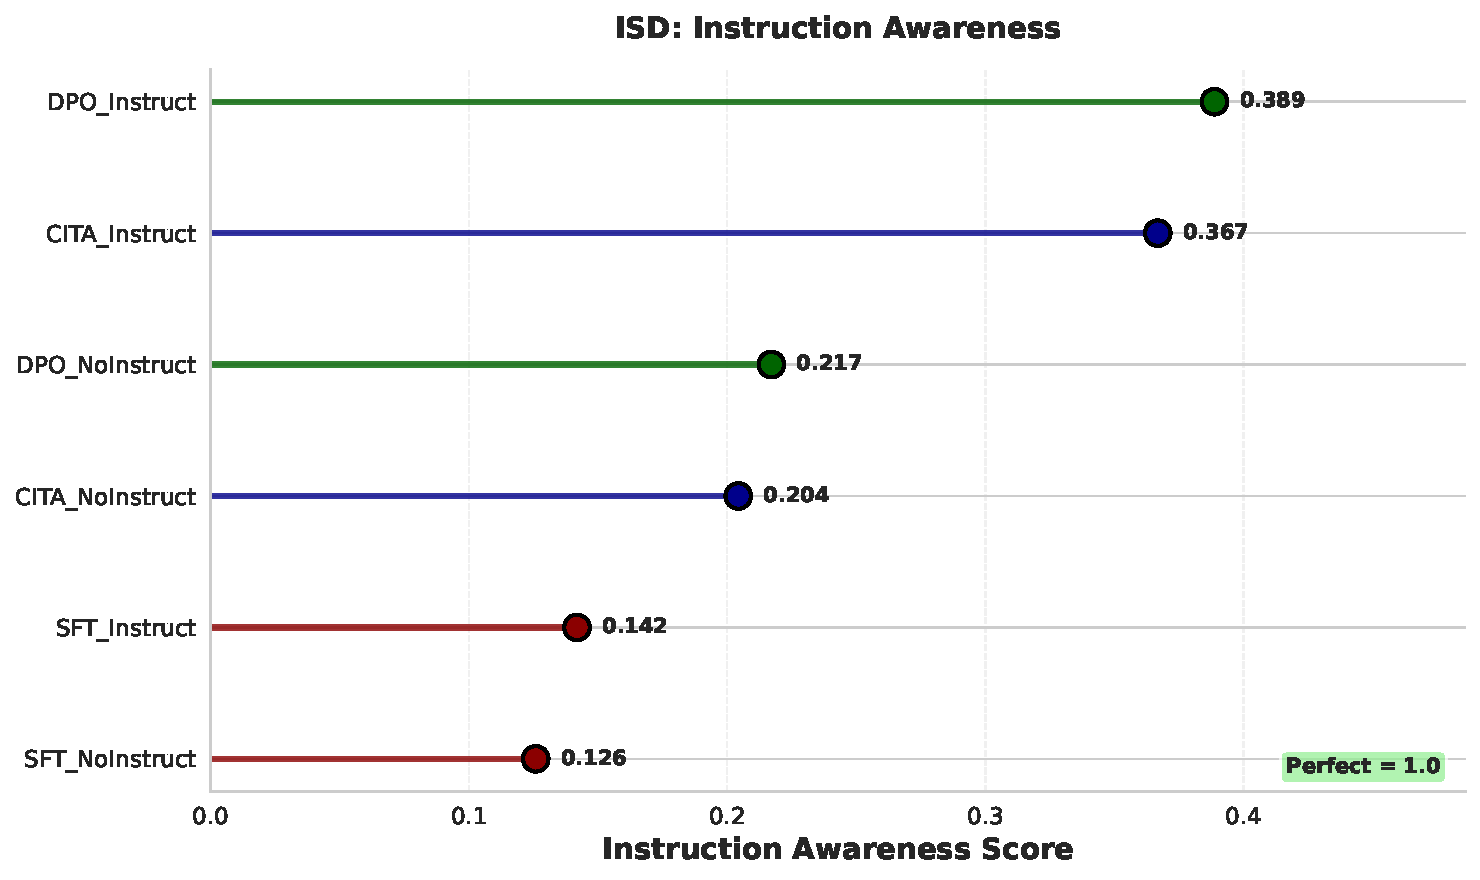
\includegraphics[width=0.95\columnwidth]{figures/evaluation/isd_comparison_lollipop.pdf}
% \caption{\textbf{ISD Lollipop}: Instruction sensitivity scores with emphasis on relative differences.}
% \label{fig:isd_lollipop}
% \vspace{-3mm}
% \end{figure}

\begin{figure}[H]
\centering

\includegraphics[width=0.95\columnwidth]{figures/evaluation/truthfulqa_comparison.pdf}
\caption{\textbf{TruthfulQA}: Only CITA\_Instruct (+0.013) and SFT\_Instruct (+0.012) achieve \textit{positive} adaptation scores.}
\label{fig:truthfulqa}
\vspace{-3mm}
\end{figure}

% COMMENTED OUT - lollipop variant not available in updated figures
% \begin{figure}[H]
% \centering
% 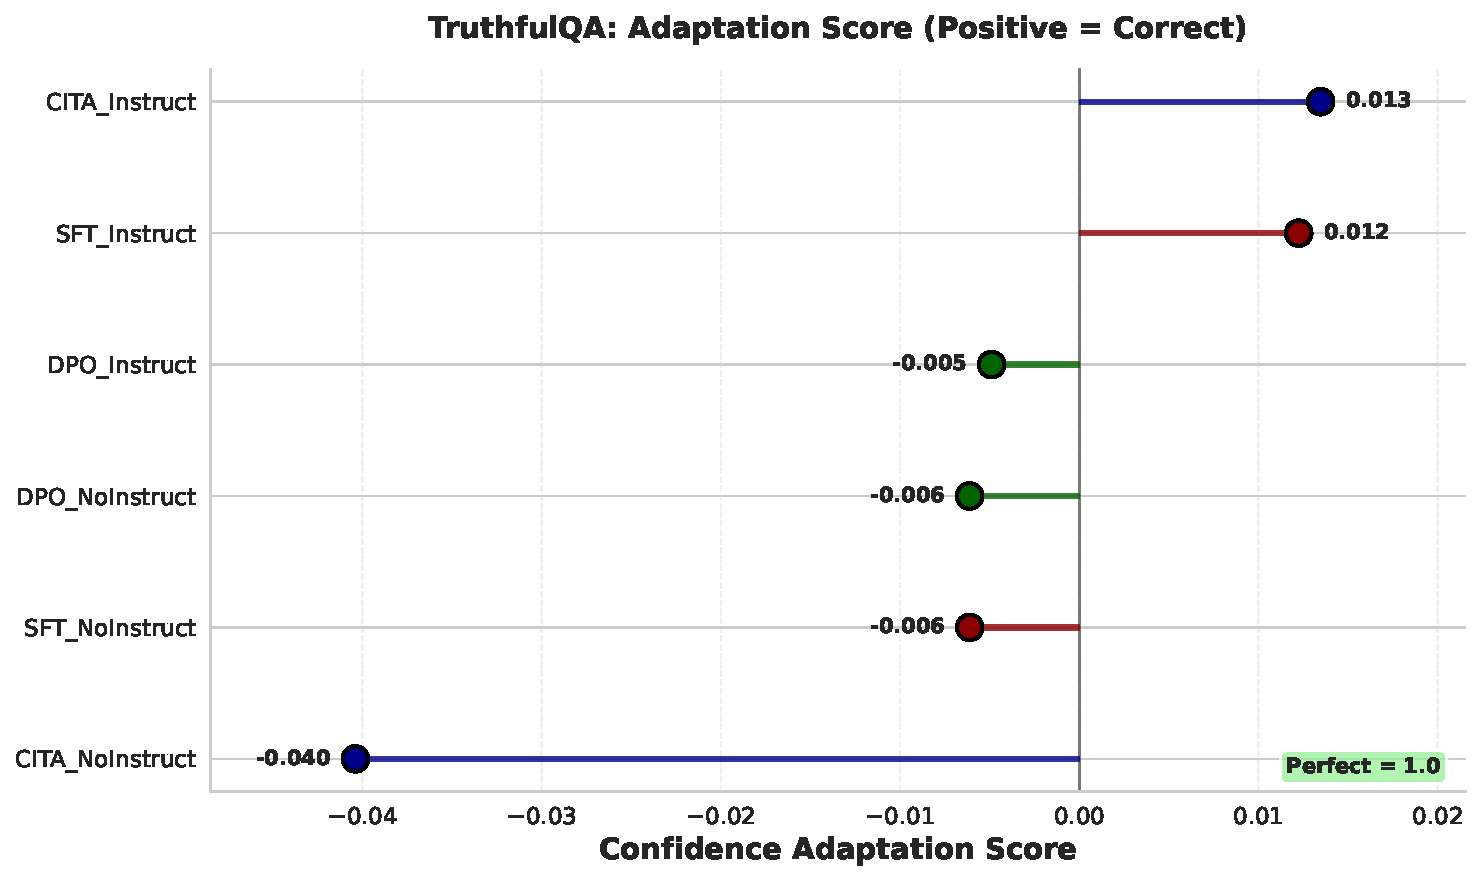
\includegraphics[width=0.95\columnwidth]{figures/evaluation/truthfulqa_comparison_lollipop.pdf}
% \caption{\textbf{TruthfulQA Lollipop}: Adaptation scores highlighting CITA's superior uncertainty calibration.}
% \label{fig:truthfulqa_lollipop}
% \vspace{-3mm}
% \end{figure}

\begin{figure}[H]
\centering

\includegraphics[width=0.95\columnwidth]{figures/evaluation/conditional_safety_comparison.pdf}
\caption{\textbf{Conditional Safety}: DPO\_Instruct (0.489) and CITA\_Instruct (0.400) show behavioral gap between STRICT vs. PERMISSIVE.}
\label{fig:conditional_safety}
\vspace{-3mm}
\end{figure}

% COMMENTED OUT - lollipop variant not available in updated figures
% \begin{figure}[H]
% \centering
% 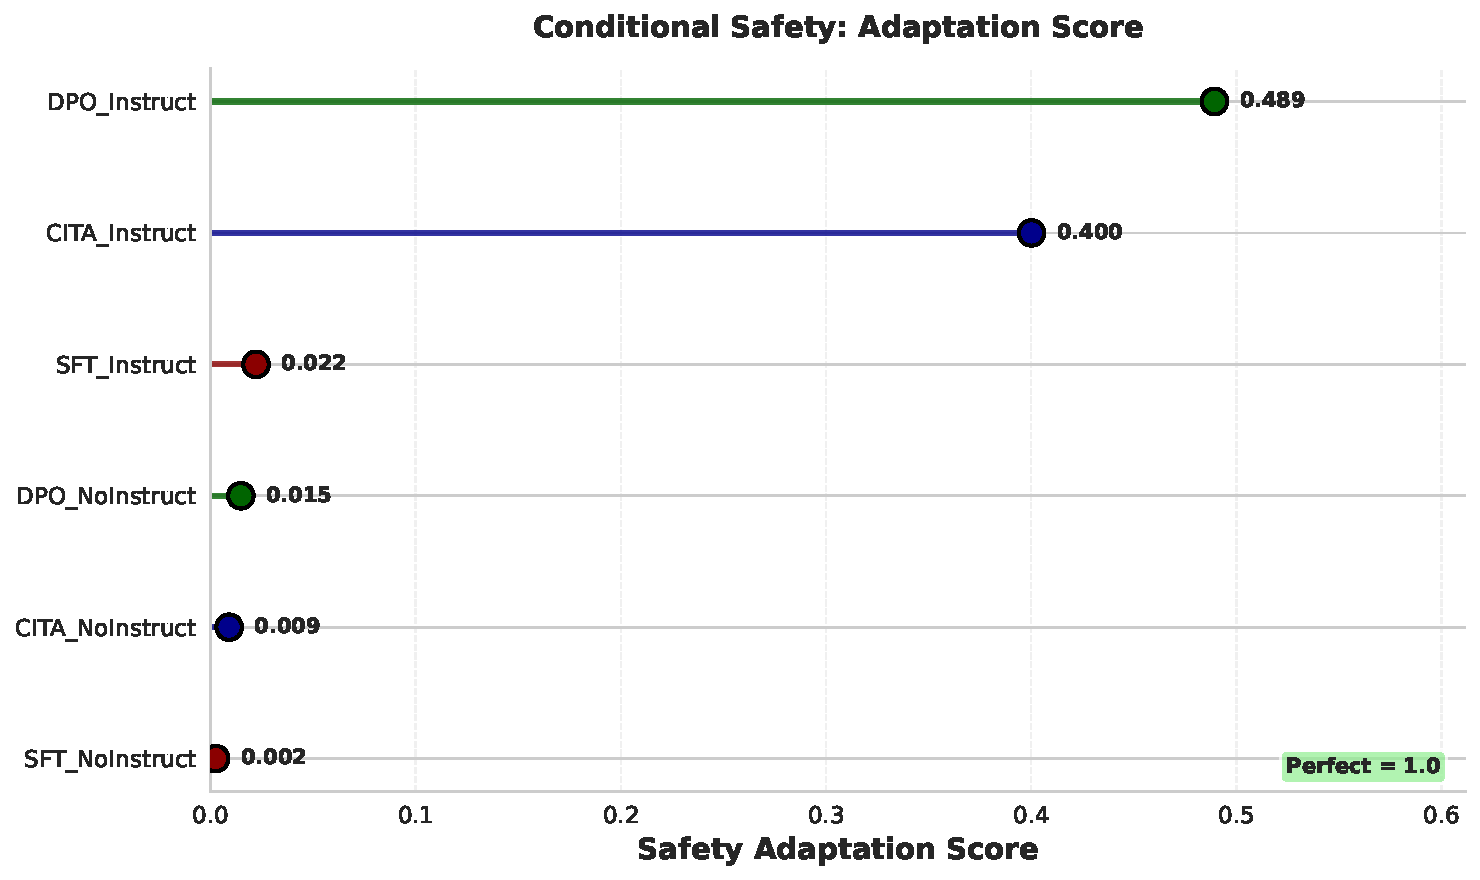
\includegraphics[width=0.95\columnwidth]{figures/evaluation/conditional_safety_comparison_lollipop.pdf}
% \caption{\textbf{Conditional Safety Lollipop}: Safety adaptation scores across STRICT vs. PERMISSIVE contexts.}
% \label{fig:conditional_safety_lollipop}
% \vspace{-3mm}
% \end{figure}

\begin{figure}[H]
\centering

\includegraphics[width=0.95\columnwidth]{figures/evaluation/length_control_comparison.pdf}
\caption{\textbf{Length Control}: CITA\_Instruct valid-only (1.77) shows strongest adaptation.}
\label{fig:length_control}
\vspace{-3mm}
\end{figure}

% COMMENTED OUT - lollipop variant not available in updated figures
% \begin{figure}[H]
% \centering
% 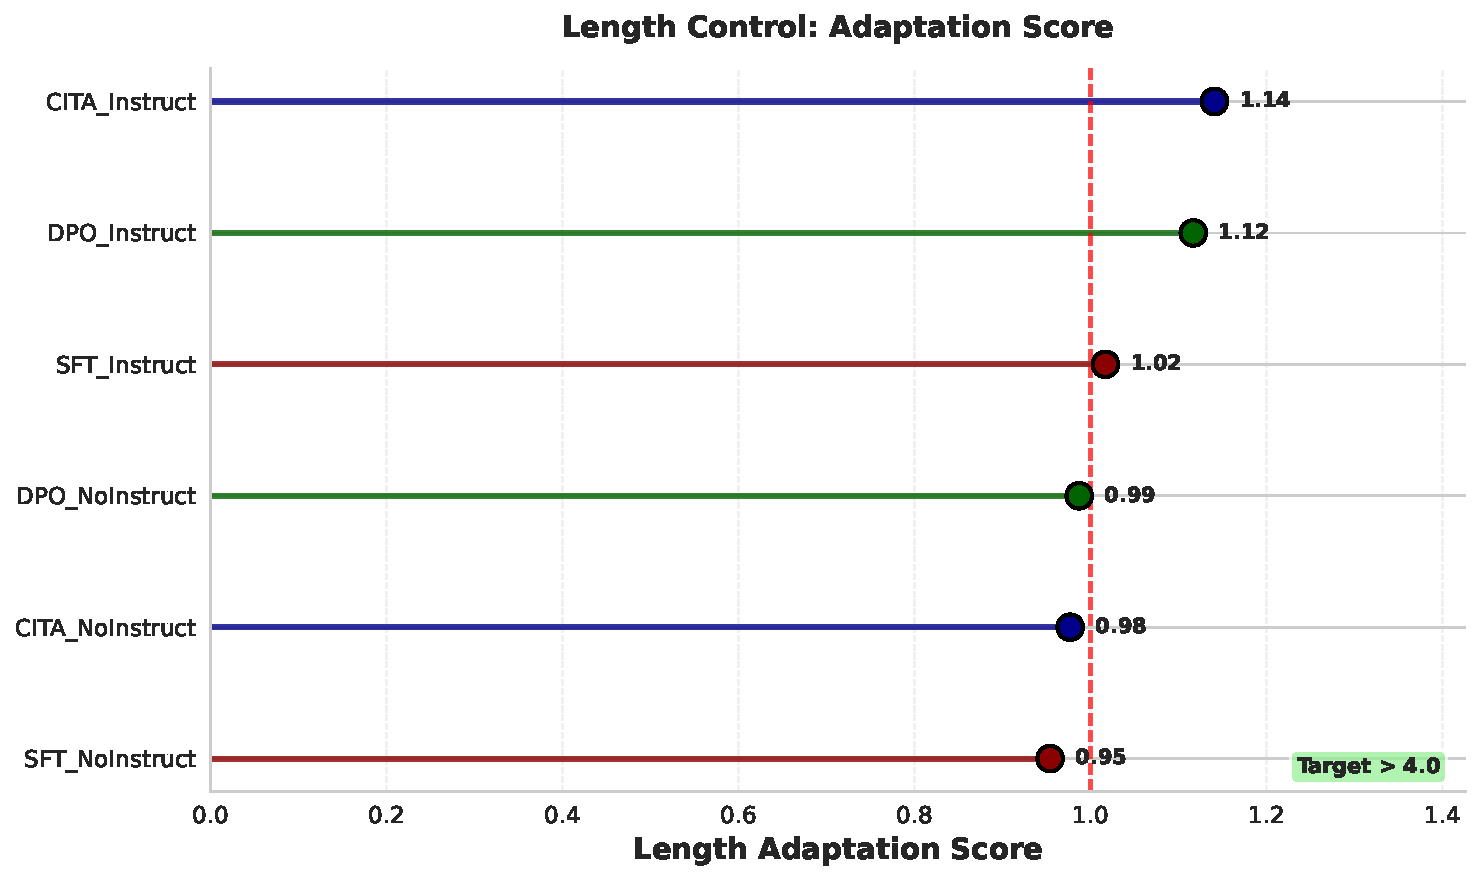
\includegraphics[width=0.95\columnwidth]{figures/evaluation/length_control_comparison_lollipop.pdf}
% \caption{\textbf{Length Control Lollipop}: Response length adaptation ratios with baseline reference.}
% \label{fig:length_control_lollipop}
% \vspace{-3mm}
% \end{figure}

\begin{figure}[H]
\centering

\includegraphics[width=0.95\columnwidth]{figures/evaluation/aqi_comparison.pdf}
\caption{\textbf{AQI}: CITA\_Instruct (55.5) and DPO\_Instruct (55.0) achieve highest clustering scores.}
\label{fig:aqi}
\vspace{-3mm}
\end{figure}

% COMMENTED OUT - lollipop variant not available in updated figures
% \begin{figure}[H]
% \centering
% 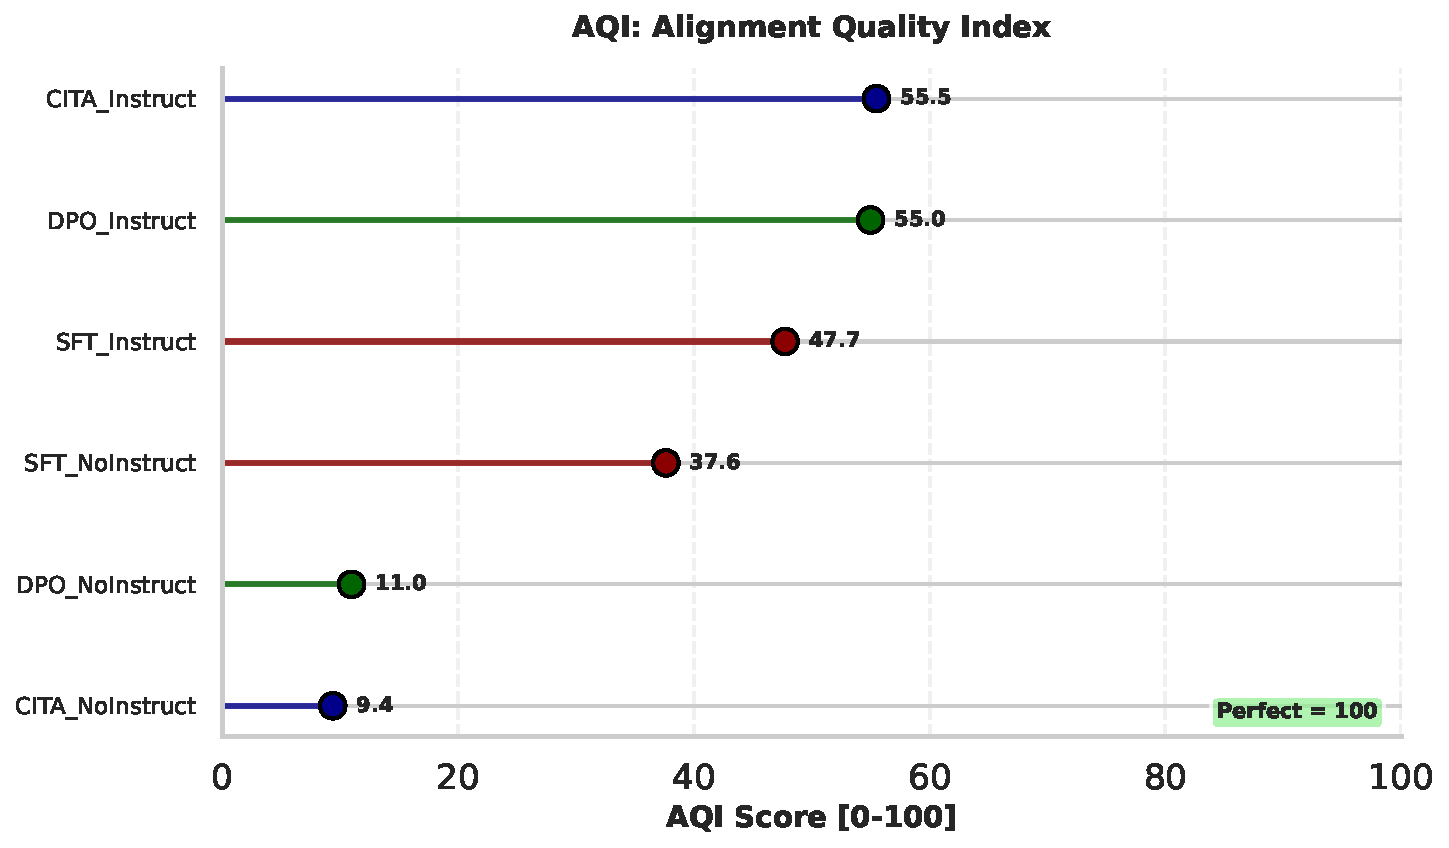
\includegraphics[width=0.95\columnwidth]{figures/evaluation/aqi_comparison_lollipop.pdf}
% \caption{\textbf{AQI Lollipop}: Alignment quality scores emphasizing CITA and DPO performance gap.}
% \label{fig:aqi_lollipop}
% \vspace{-3mm}
% \end{figure}

\vspace{-2mm}
\subsection{Combined Analysis}
\label{sec:combined_analysis}



\begin{figure}[H]
\centering

\includegraphics[width=0.95\columnwidth]{figures/evaluation/combined_plots/heatmap.pdf}
\caption{\textbf{Performance Heatmap}: Original scores with column-normalized colors. Green = best, red = worst.}
\label{fig:heatmap}
\vspace{-3mm}
\end{figure}

\vspace{-2mm}
\subsection{Key Insights}
\label{sec:key_insights}

\paragraph{TruthfulQA is the Differentiator.} On TruthfulQA, CITA improves by +0.054 (becoming appropriately more/less confident when instructed), while DPO shows negligible change (+0.001). This demonstrates CITA's superior ability to \textit{internalize} uncertainty calibration instructions.

\paragraph{CITA Achieves Higher Margins with Lower Accuracy.} Despite similar training accuracy ($\sim$89\%), CITA achieves higher reward margins (7.5 vs. 6.0). This validates that mandatory KL prevents margin collapse while enabling stable behavioral switching.

\paragraph{Instruction-Alignment $\neq$ Instruction-Following.} DPO\_I achieves higher absolute ISD scores, but CITA\_I shows more consistent improvement across diverse benchmarks. This suggests CITA achieves \textit{deeper} instruction-alignment rather than surface-level following.
